\documentclass[../main.tex]{subfiles}
\begin{document}
\chapter{Validazione del framework}
In questo capitolo verrà proposta una validazione di un deployment di test del framework Moon Cloud, mediante la valutazione della sicurezza tramite l'esecuzione del driver sviluppato a tutti i livelli dello stack cloud (infrastruttura, piattaforma, software). 

\section{Deployment di Moon Cloud}

Il deployment dell'ambiente di test è stato effettuato su un'architettura multi-layer così composta:
\begin{itemize}
    \item A livello di infrastruttura, un nodo fisico, Dell PowerEdge T430 equipaggiato con processore Intel(R) Xeon(R) CPU E5-2630 v4 (10 core fisici e 40 thread logici), 48GB di RAM e 5 dischi da 1TB ciascuno in configurazione RAID 1. Su questa macchina è stato installato il sistema operativo CentOS 7.2, e il software Open Stack Newton.
        Successivamente sono state create 3 macchine virtuali con sistema operativo CentOS 7.2, in un flavor con 4GB di RAM e 10GB di disco.
    \item A livello di piattaforma, un cluster Docker Swarm di 2 nodi per i componenti core di Moon Cloud. La terza macchina virtuale è stata utilizzata come nodo di esecuzione per un cluster di dimensione unaria.
    \item A livello software, i componenti di Moon Cloud: 7 servizi core, gestiti tramite container Docker sul cluster swarm e 3 microservizi per la gestione del nodo di esecuzione.\\
        \textbf{Componenti Core}
        \begin{itemize}
            \item API
            \item Database
            \item Repository
            \item Database dei risultati
            \item Evaluation Manager
            \item Meccanismo di comunicazione basato su code
            \item Reverse proxy
        \end{itemize}
        \textbf{Componenti execution node e execution cluster}
        \begin{itemize}
            \item Execution Manager
            \item Monitor Execution Manager
            \item Traefik (reverse proxy) per l'esposizione del servizio web \textit{Survey}
        \end{itemize}
\end{itemize}


\section{Sicurezza del deployment}
L'analisi della sicurezza è stata effettuata a livello di infrastruttura, analizzando le configurazioni sul sistema operativo del server fisico e le caratteristiche del setup OpenStack; a livello di piattaforma, analizzando le configurazioni del template utilizzato per le macchine virtuali Docker e i container Moon Cloud; a livello applicativo, analizzando la sicurezza nei meccanismi di integrazione dei vari componenti.
\subsection{Infrastruttura}
\subsubsection{Analisi OpenSCAP del server fisico}
\begin{comment}
test finished
started at 1496183480
ended at   1496184352
lasted -872 seconds
report available at
https://moonclouddashboard.blob.core.windows.net/pdfcontainer/f4a1943cff

\end{comment}
Il test è stato eseguito utilizzando il driver realizzato, specificando in input il documento XCCDF "\textit{ssg-centos7}" unitamente al profilo "\textit{nist-800-171-cui}".
Il documento \textit{JSON} dato in input al test è il seguente:
\begin{js}
{
    "read_ssh_configuration": {
    },
    "read_xccdf_configuration": {
        "xccdf":"ssg-centos7",
        "profile":"nist-800-171-cui",
        "fetch_remote_resources": true
    },
    "read_azure_configuration": {
    }
}
\end{js}

I risultati restituiti in output segnalano:
\begin{itemize}
    \item 119 valutazioni effettuate con successo
    \item 72 valutazioni fallite
\end{itemize}
\begin{figure}[H]
    \centering
    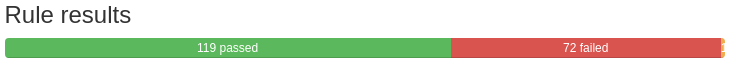
\includegraphics[width=15cm]{immagini/test_oscap_1.png}
\end{figure}

In particolare, delle 72 valutazioni fallite, 11 sono state catalogate da OpenSCAP con \textit{severity} bassa, 50 con \textit{severity} media e 11 con \textit{severity} elevata; lo score della copertura XCCDF ottenuto è 71.17\%.
\vfill\newpage
\subsubsection{Risultato del test: valutazioni fallite}
\begin{ltabulary}{|p{10cm}|p{5cm}|}
    \hline
    \textbf{Descrizione} & \textbf{Security Control}
    \\ \hline
    \endhead

Allow Only SSH Protocol 2                                                             & AC-17, IA-5 \\ \hline
Build and Test AIDE Database                                                          & CM-3(d), CM-3(e), CM-6(d), CM-6(3), SC-28, SI-7 \\ \hline
Configure AIDE to Use FIPS 140-2 for Validating Hashes                                & SI-7(1) \\ \hline
Configure AIDE to Verify Access Control Lists (ACLs)                                  & SI-7.1 \\ \hline
Configure AIDE to Verify Extended Attributes                                          & SI-7.1 \\ \hline
Configure Notification of Post-AIDE Scan Details                                      & CM-3(5)  \\ \hline
Configure Periodic Execution of AIDE                                                  & CM-3(d), CM-3(e), CM-3(5), CM-6(d), CM-6(3), SC-28, SI-7 \\ \hline
Configure the root Account for failed Password Attempts                               & AC-7(b) \\ \hline
Direct root Logins Not Allowed                                                        & IA-2(1) \\ \hline
Disable Compression Or Set Compression to delayed                                     & CM-6(b) \\ \hline
Disable Ctrl-Alt-Del Reboot Activation                                                & AC-6 \\ \hline
Disable GSSAPI Authentication                                                         & CM-6(c) \\ \hline
Disable KDump Kernel Crash Analyzer (kdump)                                           & AC-17(8), CM-7, CM-6(b) \\ \hline
Disable Kerberos Authentication                                                       & CM-6(c) \\ \hline
Disable Prelinking                                                                    & CM-6(c) \\ \hline
Disable SSH Access via Empty Passwords                                                & AC-3, AC-6, CM-6(b) \\ \hline
Disable SSH Root Login                                                                & AC-3, AC-17(2), AU-10(5), CM-6(b), IA-5(1)(c), IA-7 \\ \hline
Disable SSH Support for Rhosts RSA Authentication                                     & AC-3, AC-6, CM-6(b) \\ \hline
Disable SSH Support for User Known Hosts                                              & CM-6(a) \\ \hline
Disable Support for RPC IPv6                                                          & CM-6(a) \\ \hline
Disable xinetd Service                                                                & AC-17(8), CM-7 \\ \hline
Do Not Allow SSH Environment Options                                                  & CM-6(b)  \\ \hline
Enable Smart Card Login                                                               & IA-2(2) \\ \hline
Enable SSH Warning Banner                                                             & AC-8(a), AC-8(b), AC-8(c)(1), AC-8(c)(2), AC-8(c)(3) \\ \hline
Enable Use of Privilege Separation                                                    & AC-6 \\ \hline
Enable Use of Strict Mode Checking                                                    & AC-6 \\ \hline
Ensure gpgcheck Enabled For All Yum Package Repositories                              & CM-5(3), SI-7, MA-1(b) \\ \hline
Ensure gpgcheck Enabled for Local Packages                                            & CM-5(3) \\ \hline
Ensure gpgcheck Enabled for Repository Metadata                                       & CM-5(3) \\ \hline
Ensure Logs Sent To Remote Host                                                       & AU-3(2), AU-4(1), AU-9 \\ \hline
Ensure System is Not Acting as a Network Sniffer                                      & CM-7, CM-7(2).1(i) \\ \hline
Ensure the Logon ure Delay is Set Correctly in login.defs                             & IA-5(f), IA-5(1)(a) \\ \hline
Ensure YUM Removes Previous Package Versions                                          & SI-2 \\ \hline
Install AIDE                                                                          & CM-3(d), CM-3(e), CM-6(d), CM-6(3), SC-28, SI-7 \\ \hline
Install the dracut-fips Package                                                       & AC-17(2) \\ \hline
Install Virus Scanning Software                                                       & SC-28, SI-3 \\ \hline
Limit Password Reuse                                                                  & IA-5(1)(e) \\ \hline
Limit the Number of Concurrent Login Sessions Allowed Per User                        & AC-10  \\ \hline
Modify the System Login Banner                                                        & AC-8(a), AC-8(b), AC-8(c)(1), AC-8(c)(2), AC-8(c)(3) \\ \hline %
Prevent Log In to Accounts With Empty Password                                        & AC-6, IA-5(b), IA-5(c), IA-5(1)(a) \\ \hline
Restrict Serial Port Root Logins                                                      & AC-6(2) \\ \hline
Restrict Virtual Console Root Logins                                                  & AC-6(2) \\ \hline
Set Account Expiration Foling Inactivity                                              & AC-2(2), AC-2(3), IA-4(e) \\ \hline
Set Deny For failed Password Attempts                                                 & AC-7(b) \\ \hline
Set Interactive Session Timeout                                                       & AC-12, SC-10 \\ \hline
Set Interval For Counting ed Password Attempts                                        & AC-7(b) \\ \hline
Set Lockout Time For ed Password Attempts                                             & AC-7(b) \\ \hline
Set Password Maximum Age                                                              & IA-5(b), IA-5(c), IA-5(1)(a) \\ \hline
Set Password Maximum Consecutive Repeating Characters                                 & IA-5(b), IA-5(c), IA-5(1)(a) \\ \hline
Set Password Minimum Age                                                              & IA-5(b), IA-5(c), IA-5(1)(a) \\ \hline
Set Password Minimum Length                                                           & IA-5(b), IA-5(c), IA-5(1)(a) \\ \hline
Set Password Minimum Length in login.defs                                             & IA-5(b), IA-5(c), IA-5(1)(a) \\ \hline
Set Password Retry Prompts Permitted PSession                                         & IA-5(b), IA-5(c), IA-5(1)(a) \\ \hline
Set Password Strength Minimum Different Categories                                    & IA-5(b), IA-5(c), IA-5(1)(a) \\ \hline
Set Password Strength Minimum Different Characters                                    & IA-5(b), IA-5(c), IA-5(1)(a) \\ \hline
Set Password Strength Minimum Digit Characters                                        & IA-5(b), IA-5(c), IA-5(1)(a) \\ \hline
Set Password Strength Minimum Special Characters                                      & IA-5(b), IA-5(c), IA-5(1)(a) \\ \hline
Set Password Strength Minimum Uppercase Characters                                    & IA-5(b), IA-5(c), IA-5(1)(a) \\ \hline
Set Password to Maximum of Consecutive Repeating Characters from Same Character Class & IA-5(b), IA-5(c), IA-5(1)(a) \\ \hline
Set SSH Client Alive Count                                                            & AC-2(5), SA-8, AC-12 \\ \hline
Set SSH Idle Timeout Interval                                                         & AC-7(b) \\ \hline
The Installed Operating System Is Vendor Supported and Certified                      & SI-2(c) \\ \hline
Uninstall xinetd Package                                                              & AC-17(8), CM-7 \\ \hline
Use Only FIPS 140-2 Validated Ciphers                                                 & AC-3, AC-17(2), AU-10(5), CM-6(b), IA-5(1)(c), IA-7 \\ \hline
Use Only FIPS 140-2 Validated MACs                                                    & AC-17(2), IA-7, SC-13 \\ \hline
Verify and Correct File Permissions with RPM                                          & AC-6, AU-9(1), AU-9(3), CM-6(d), CM-6(3) \\ \hline
Verify File Hashes with RPM                                                           & CM-6(d), CM-6(3), SI-7(1) \\ \hline
Verify firewalld Enabled                                                              & CM-6(b) \\ \hline

\end{ltabulary}
\begin{figure}[H]
    \centering
    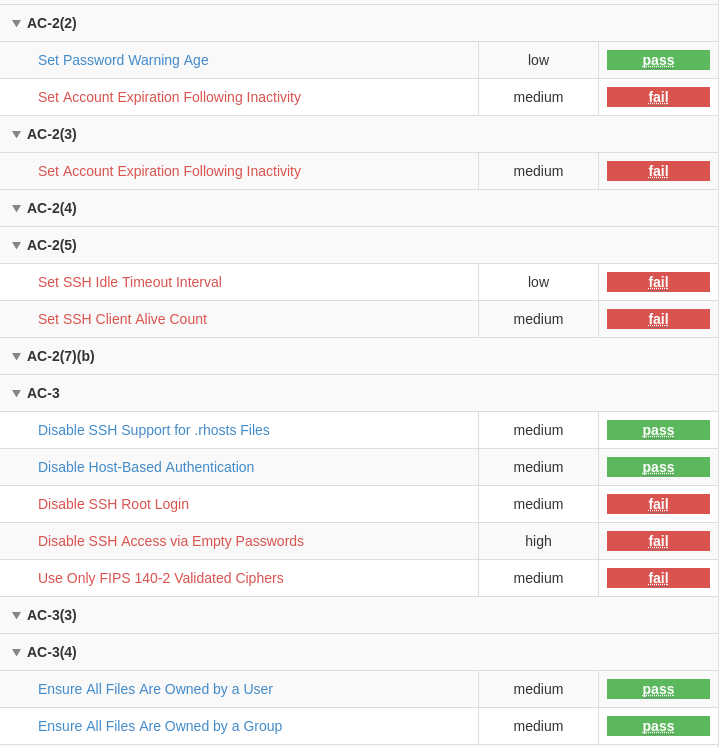
\includegraphics[width=10cm]{immagini/test_oscap_1_1.png}
    \caption{Estratto del report}\label{ref:report_oscap_1_1}
\end{figure}
    
In figura \ref{ref:report_oscap_1_1} è riportata una parte del report generato dal controllo sviluppato. Esso, in formato HTML, contiene il riepilogo di tutti i test eseguiti con il relativo stato e gli script di \textit{remediation}. Il documento completo è disponibile in formato HTML all'indirizzo:\\
\textit{https://moonclouddashboard.blob.core.windows.net/pdfcontainer/f4a1943cff}
\\
o nel repository GIT\\
\textit{https://github.com/patriziotufarolo/tesi\_magistrale/}.

La valutazione delle \textit{OVAL} mediante il driver realizzato è durata 872 secondi; di seguito sono riportate le statistiche relative all'utilizzo delle risorse nell'esecuzione del test.
Queste sono state raccolte tramite il software \texttt{pidstat}, isolando esclusivamente i processi coinvolti nel processo di assessment.
\begin{figure}[H]
 \begin{minipage}[b]{6cm}
   \centering
   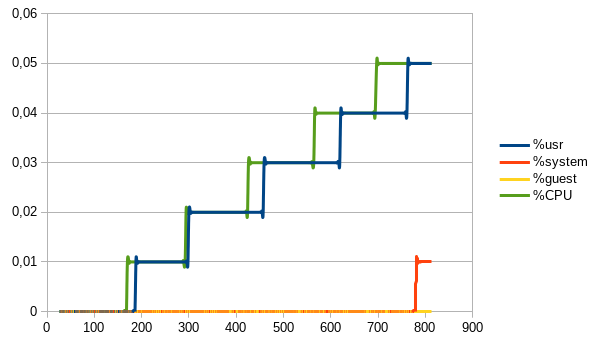
\includegraphics[width=6.6cm]{immagini/plot1cpu.png}
 \end{minipage}
 \hspace{2mm} \hspace{3mm}
 \begin{minipage}[b]{9cm}
  \centering
   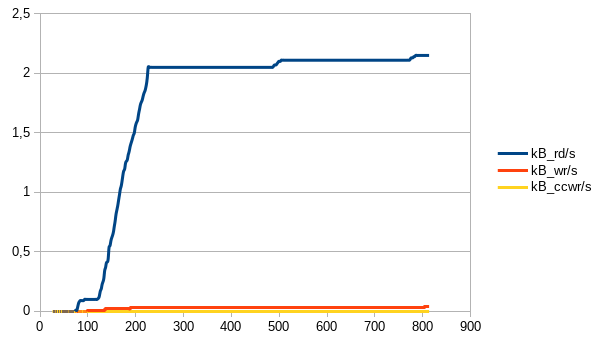
\includegraphics[width=6.6cm]{immagini/plot1io.png}
 \end{minipage}
 \caption{Utilizzo della CPU e carico IO}\label{ref:plot1cpuio}
\end{figure}
Dalla figura \ref{ref:plot1cpuio} è possibile notare come l'impatto del test sulle prestazioni del target sia minimo, registrando picchi di carico sulla CPU inferiori all'0.06\% per tutta la durata dell'esecuzione. Anche dal punto di vista delle operazioni di input/output il test si è dimostrato assolutamente non invasivo, registrando picchi in lettura di pochi KB. 
\begin{figure}[H]
 \begin{minipage}[b]{6cm}
   \centering
   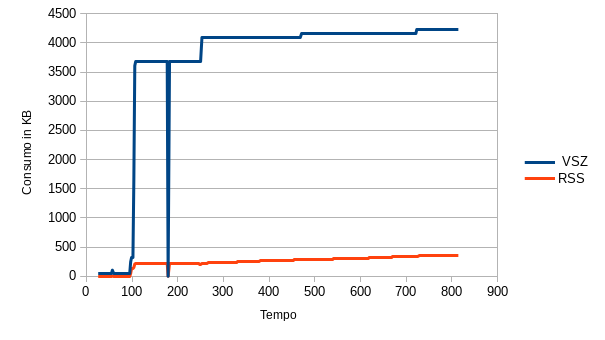
\includegraphics[width=6.6cm]{immagini/plot1mem.png}
 \end{minipage}
 \hspace{2mm} \hspace{3mm}
 \begin{minipage}[b]{9cm}
  \centering
   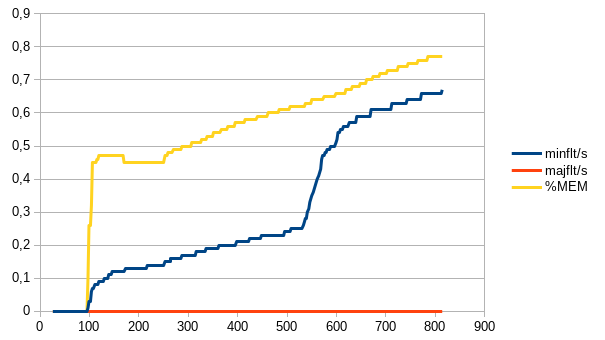
\includegraphics[width=6.6cm]{immagini/plot1mem2.png}
 \end{minipage}
 \caption{Utilizzo della memoria}\label{ref:plot1mem}
\end{figure}
In figura \ref{ref:plot1mem} è stato invece illustrato l'utilizzo della memoria durante l'esecuzione del test, che rimane sempre inferiore all'1\%. Anche in questo caso l'impatto prestazionale è minimo; il \textit{footprint} di \textit{OpenSCAP} e delle relative \textit{probes} non raggiunge i 5MB in memoria virtuale (\textit{VSZ}), rimanendo inoltre sotto i 500 KB in memoria RAM(\textit{RSS}).
Questo driver si presta particolarmente a scenari di esecuzione programmata e automatica, per effettuare monitoraggio continuativo, dimostrandosi adeguato per l'utilizzo in Moon Cloud.

\subsubsection{Analisi di OpenStack}
I documenti XCCDF forniti da OpenSCAP non sono risultati efficienti per l'assessment dei controlli di sicurezza per Open Stack, in quanto le definizioni \textit{OVAL} non sono state redatte
Questa sezione, pertanto, fa riferimento ad alcune raccomandazioni del paper "\textit{A Security Benchmark for OpenStack}" \cite{MyPaper}. Ogni raccomandazione recensita è mappata sui requisiti FedRAMP corrispondenti. A causa del fatto che l'implementazione dei controlli automatici per alcuni di queste non sono disponibili, l'analisi è stata fatta in modo manuale ispezionando le configurazioni.
Laddove è applicata la dicitura "Non applicabile", si intende che il controllo non è effettuabile nello specifico scenario valutato.
\begin{ltabulary}{|p{6cm}|p{4cm}|p{2cm}|}
    \hline
    \textbf{Reccomendation} & \textbf{FedRAMP SCs} & \textbf{Risultato} \\ \hline
    \endhead 
    {[R1]} Patch Levels                                                                              & SA-10(1), SI(3)                  & Passato         \\ \hline
    {[R2]} Create and Enforce Account and Password Management Policies                                & AC-2, AC-2(3), AC-6, AC-7, AC-9  & Fallito         \\ \hline
    {[R3]} Use a Central Directory for Authentication and Authorization.                              & AC-3, AC-17                      & Fallito         \\ \hline
    {[R4]} Configure Firewalls to Restrict Access                                                     & CM-6, CM-7                       & Passato         \\ \hline
    {[R5]} Use TLS/SSL where Possible                                                                 & AC-3, AC-17(2), AU-10(5), CM-6(b), IA-5(1)(c), IA-7 & Fallito  \\ \hline
    {[R6]} Do Not Use Default Self-Signed Certificates.                                               & AC-3, AC-17(2), AU-10(5), CM-6(b), IA-5(1)(c), IA-7 & Non Applicabile \\ \hline
    {[R7]} Configure Centralized Remote Logging                                                       & AU-3(2), AU-4(1), AU-9           & Fallito         \\ \hline
    {[R8]} Maintain Time Synchronization Services                                                     & AU-8                             & Passato         \\ \hline
    {[R11]} Use Templates to Deploy Virtual Machines                                                  & -                                & Passato         \\ \hline
    {[R13]} Disable MAC Address Changes and Promiscuous Mode on Guests                                & CM-7, CM-7(2).1(i)               & Passato         \\ \hline
    {[R14]} Ensure Network Isolation through VLANs                                                    & SC-2, SC-7, SC-8                 & Passato         \\ \hline
    {[R15]} Port Groups Should not be Configured to Reserved VLANs                                    & CM-7                                & Passato         \\ \hline
    {[R16]} Secure Access to Cloud Application Programming Interfaces                                 & CM-7                                & Fallito         \\ \hline
    {[R17]} Encrypt Data at Rest                                                                      & SC-28, SC-28 (1)                & Fallito         \\ \hline
    {[R18]} Establish Appropriate Resource Isolation                                                  & SC-39                           & Passato         \\ \hline
    {[R19]} Evaluate Denial of Service Scenarios and Mitigations                                      & SC-06                            & Fallito         \\ \hline
    {[R20]} Do Not Use or Set Guest Customization Passwords                                           & IA-5(7)                          & Passato         \\ \hline
    {[R22]} Audit Sensible and Configuration Files                                                    & AU-3, AU-8, AU-12                & Fallito         \\ \hline
    {[R23]} Storage Reliability                                                                       & CP-4, CP-9                       & Fallito         \\ \hline
    {[R24]} Data Remanence Avoidance                                                                  & SC-4                             & Fallito         \\ \hline
\end{ltabulary}
Il 55\% delle valutazioni ha avuto esito negativo sull'ambiente di sviluppo, in quanto esso non è ovviamente predisposto per essere utilizzato in scenari di produzione.
Nel caso in cui \textit{Moon Cloud} vorrà ricevere l'autorizzazione provvisoria ad operare dalla JBO FedRAMP è ovviamente necessario che sia installato su un provider \textit{IaaS} autorizzato (ad esempio Microsoft Azure).

\subsection{Piattaforma}
\subsubsection{Analisi OpenSCAP sul template delle macchine virtuali}
Il test con il driver OpenSCAP è stato ripetuto sulle macchine virtuali dei nodi appartenenti al cluster Swarm.

I risultati restituiti in output segnalano:
\begin{itemize}
    \item 122 valutazioni effettuate con successo
    \item 69 valutazioni fallite
\end{itemize}
\begin{figure}[H]
    \centering
    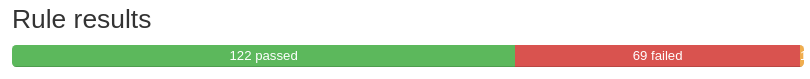
\includegraphics[width=15cm]{immagini/test_oscap_2.png}
\end{figure}

Il report completo è disponibile all'indirizzo \\
\textit{https://moonclouddashboard.blob.core.windows.net/pdfcontainer/b73210ae24}    \\   
oppure \\
\textit{https://www.github.com/patriziotufarolo/tesi\_magistrale/} \\


\begin{comment}
test finished
started at 1496218136
ended at 1496218350
lasted -214 seconds

report available at
https://moonclouddashboard.blob.core.windows.net/pdfcontainer/b73210ae24
--
\end{comment}
\subsubsection{Analisi del cluster Docker Swarm}
L'analisi del cluster Swarm è stata condotta utilizzando lo strumento \textit{Docker Security Benchmark}\footnote{Docker Security Benchmark - \textit{https://www.dockerbench.com}}.
Di seguito è proposto un mapping tra le verifiche fallite e i controlli di sicurezza FedRAMP non rispettati; per motivi di proprietà intellettuale i nomi di alcuni container sono stati oscurati.
    \begin{ltabulary}{|p{9cm}|p{5cm}|}
        \hline
        \textbf{Controllo} & \textbf{FedRAMP SCs} \\
        \hline
        \endhead

Audit docker daemon - /usr/bin/docker                                                                                                                                                                                                                                                       & AU-3, AU-8, AU-12                                   \\ \hline
Audit Docker files and directories - /var/lib/docker, /etc/docker, docker.service, /docker-containerd, docker-runc                                                                                                                                                                          & AU-3, AU-8, AU-12                                   \\ \hline
Restrict network traffic between containers                                                                                                                                                                                                                                                 & SC-2, SC-7, SC-8                                    \\ \hline
Docker daemon currently listening on TCP without TLS                                                                                                                                                                                                                                        & AC-3, AC-17(2), AU-10(5), CM-6(b), IA-5(1)(c), IA-7 \\ \hline
Enable user namespace support                                                                                                                                                                                                                                                               & AC-4(21), AC-5, AC-6 (01), AC-6(02), AC-6(05)       \\ \hline
Use authorization plugin                                                                                                                                                                                                                                                                    & AC-3 AC-4                                                    \\ \hline
Configure centralized and remote logging                                                                                                                                                                                                                                                    & AU-3(2), AU-4(1), AU-9                           \\ \hline
Disable operations on legacy registry (v1)                                                                                                                                                                                                                                                  & -                                                 \\ \hline
Bind swarm services to a specific host interface                                                                                                                                                                                                                                            & SC-2, SC-7, SC-8, SC-10                                                     \\ \hline
Unencrypted overlay network: ingress (swarm), mooncloud (swarm)                                                                                                                                                                                                                             & SC-8, SC-8(1), SC-10                                                     \\ \hline
Run swarm manager in auto-lock mode                                                                                                                                                                                                                                                         & SC-27                                               \\ \hline
Create a user for the container                                                                                                                                                                                                                                                             &  AC-4(21), AC-5, AC-6 (01), AC-6(02), AC-6(05)                                                     \\ \hline
Running as root:  mooncloud\_evaluationmodule, mooncloud\_api, mooncloud\_traefik, mooncloud\_monitor\_execution\_manager, mooncloud\_dashboard, mooncloud\_*********, mooncloud\_***********, mooncloud\_db, mooncloud\_******, mooncloud\_execution\_manager                              &  AC-4(21), AC-5, AC-6 (01), AC-6(02), AC-6(05)                                                   \\ \hline
Enable Content trust for Docker:  mooncloud\_evaluationmodule, mooncloud\_api, mooncloud\_traefik, mooncloud\_monitor\_execution\_manager, mooncloud\_dashboard, mooncloud\_*********, mooncloud\_***********, mooncloud\_db, mooncloud\_******, mooncloud\_execution\_manager              &                                                     \\ \hline
No AppArmorProfile Found:   mooncloud\_evaluationmodule, mooncloud\_api, mooncloud\_traefik, mooncloud\_monitor\_execution\_manager, mooncloud\_dashboard, mooncloud\_*********, mooncloud\_***********, mooncloud\_db, mooncloud\_******, mooncloud\_execution\_manager                    &                                                     \\ \hline
No selinux SecurityOptions Found:  mooncloud\_evaluationmodule, mooncloud\_api, mooncloud\_traefik, mooncloud\_monitor\_execution\_manager, mooncloud\_dashboard, mooncloud\_*********, mooncloud\_***********, mooncloud\_db, mooncloud\_******, mooncloud\_execution\_manager             &                                                     \\ \hline
Container running with root FS mounted R/W:  mooncloud\_evaluationmodule, mooncloud\_api, mooncloud\_traefik, mooncloud\_monitor\_execution\_manager, mooncloud\_dashboard, mooncloud\_*********, mooncloud\_***********, mooncloud\_db, mooncloud\_******, mooncloud\_execution\_manager   &                                                     \\ \hline

\end{ltabulary}



\subsubsection{Livello applicativo: analisi dei componenti software}

L'analisi applicativa sulla piattaforma Moon Cloud è stata svolta analizzando le configurazioni dei servizi e la loro implementazione.


Di seguito i punti critici individuati:

\subsubsection{Conclusioni}

\end{document}
